% Fig. 2 -- Consent-Aware Perception-Reasoning-Action-Consent loop
\documentclass[tikz,border=6pt]{standalone}
\usepackage{mathptmx}
\usetikzlibrary{arrows.meta,positioning,calc}
\definecolor{pf}{HTML}{F5E6F5}\definecolor{pb}{HTML}{B050C0}
\definecolor{tf}{HTML}{E0F0F0}\definecolor{tb}{HTML}{60B0B0}
\begin{document}
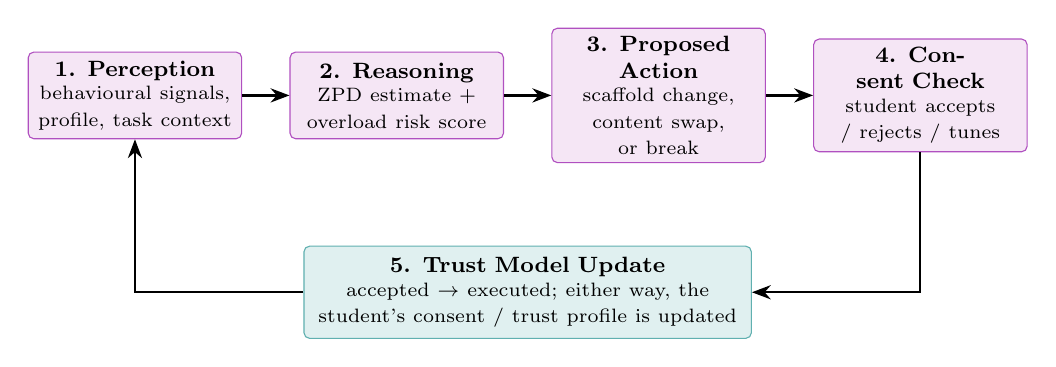
\begin{tikzpicture}[font=\footnotesize,
  st/.style={draw=pb,fill=pf,rounded corners=2pt,align=center,text width=2.5cm,minimum height=1.1cm,inner sep=3pt},
  ar/.style={-{Stealth[length=2.4mm]},thick}]
\node[st] (p) at (0,0) {\textbf{1. Perception}\\[-1pt]{\scriptsize behavioural signals, profile, task context}};
\node[st,right=0.6cm of p] (r) {\textbf{2. Reasoning}\\[-1pt]{\scriptsize ZPD estimate + overload risk score}};
\node[st,right=0.6cm of r] (a) {\textbf{3. Proposed Action}\\[-1pt]{\scriptsize scaffold change, content swap, or break}};
\node[st,right=0.6cm of a] (c) {\textbf{4. Consent Check}\\[-1pt]{\scriptsize student accepts / rejects / tunes}};
\node[draw=tb,fill=tf,rounded corners=2pt,align=center,text width=5.4cm,inner sep=4pt] (t) at ($(r)!0.5!(a)+(0,-2.5)$) {\textbf{5. Trust Model Update}\\[-1pt]{\scriptsize accepted $\rightarrow$ executed; either way, the student's consent / trust profile is updated}};
\draw[ar] (p)--(r); \draw[ar] (r)--(a); \draw[ar] (a)--(c);
\draw[ar] (c.south) |- (t.east);
\draw[ar] (t.west) -| (p.south);
\end{tikzpicture}
\end{document}
